\documentclass{article}
\usepackage{graphicx}
\usepackage{float}
\usepackage{subcaption}
\usepackage{amsmath}
\usepackage[colorlinks=true, allcolors=blue]{hyperref}

\bibliographystyle{alpha}

\title{Information Theory \\ \large Problem set 02 - Probability, entropy and inference}
\author{Luís Felipe Ramos Ferreira}
\date{\href{mailto:lframos\_ferreira@outlook.com}{\texttt{lframos\_ferreira@outlook.com}}
}

\begin{document}

\maketitle

\begin{enumerate}
	\item \begin{enumerate}
		      \item The frequentist interpretation of probability is, obviously, associated with the concept of frequency. It states that the probability \(p(s)\) of a event \(s\) should reflect the frequency that the event \(s\) happens compared to the rest of the events in the sample space, as the number of experiments goes to infinity. On the other hand, the bayesian interpretation of probability is more subjective, as it assumes the probability \(p(s)\) of a event \(s\) is the degree of belief we should have that the outcome of an experiment in the sample space will be \(s\).
		      \item Forward probability is a kind of probability in which the main goal is to "predict" the desired values. In other words, the task is to compute a probability distribution of a value, given the complete scenario of the process. As an example, given a box with \(N_b\) black balls and \(N_w\) white balls, whats the probablity distribution of the number of black balls taken frm the box, if \(N\) random balls are taken from the box, with replacement.
		            Inverse probability, just like forward probability, is a kind of probability used do "predict" the results of a given process, i.e., create a generative model of a process. But, instead of computing a probability distribution of some value of the process, it computes the conditional probability of unknown variables given the value o known variables of the process. Obviously, this kind of probability uses a lot of Bayes' theorem.
		      \item Probability is a term that can be used directed as the chance of something happening, or the degree of belief we have on something happening. The term probability can be used to describe the odds of a event in a sample space. Likelihood, on the other hand, is used to describe how well some kind of parameter describes a observed data. For example: what is the likelihood that Santa Claus was the one who gave me a present, given the fact I have a present under my Christmas tree?
	      \end{enumerate}

	\item Obviously, the probability that the first ball is white, \(P_f\), is equal to \(\frac{w}{w + b}\), since there are \(w + b\) balls and \(w\) of them are white. Let's calculate now the event of the second ball being white. We should consider that the first ball can be either white or black in this case, and each outcome for the first ball can affect the outcome for the second ball. So, we have that the probability \(P_s\) of the second ball being white is defined as the sum of the probability that the second ball is white given the fact the first ball was white and the probability that the second ball is white given that the first ball was black. In mathematical terms, it would be:
	      \begin{gather}
		      P_s = P_f\frac{w - 1}{w - 1 + b} + (1 - P_f)\frac{w}{w + b - 1} \\
		      P_s = P_f\frac{w}{w + b - 1} - \frac{P_f}{w + b - 1} + \frac{w}{w + b - 1} - P_f\frac{w}{w + b - 1} \\
		      P_s = \frac{w - P_f}{w + b - 1} \\
		      P_s = \frac{w - \frac{w}{w + b}}{w + b - 1} \\
		      P_s = \frac{w(w + b) - w}{(w + b - 1)(w + b)} \\
		      P_s = \frac{w(w + b - 1)}{(w + b - 1)(w + b)} \\
		      P_s = \frac{w}{w + b}
	      \end{gather}

	      At the end, we have what we expected, \(P_f = P_s = \frac{w}{w + b}\).

	\item Question answered by hand
	      \begin{figure}[H]
		      \centering
		      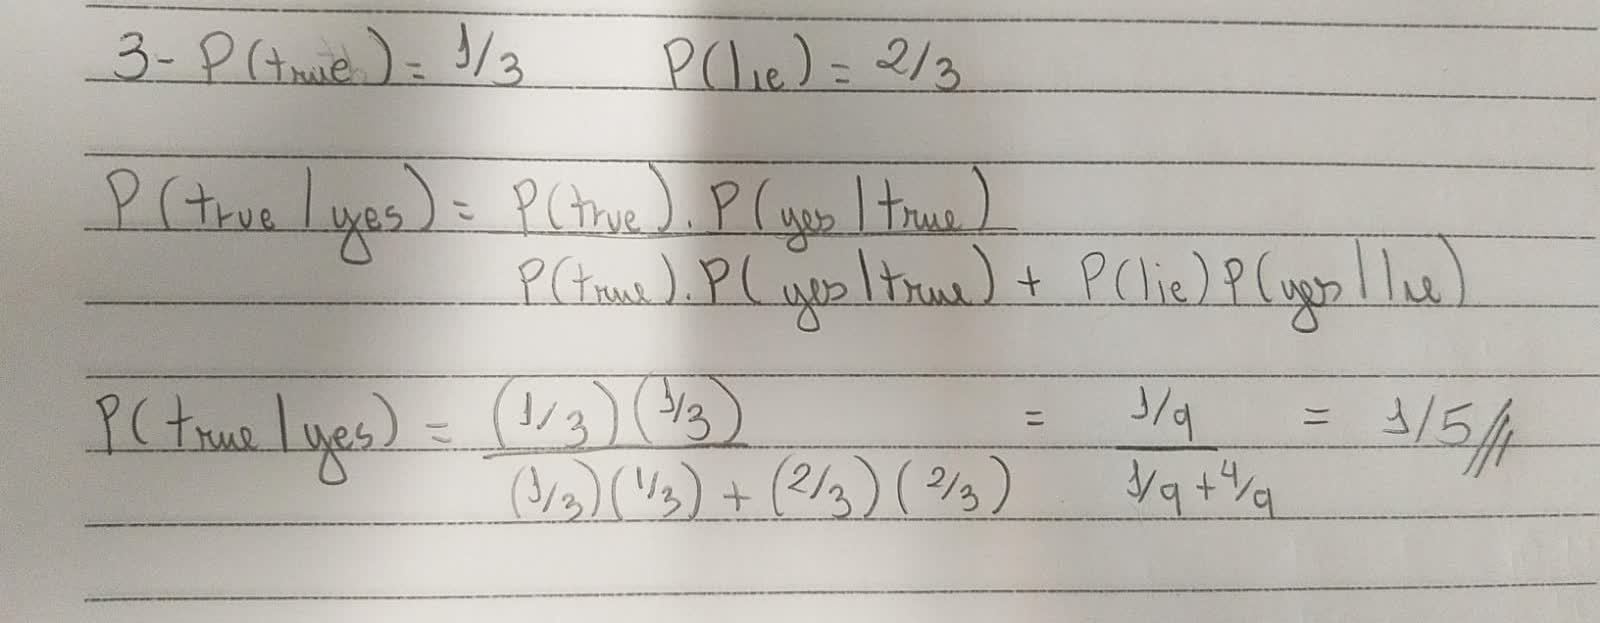
\includegraphics[width=0.5\textwidth]{images/03.jpeg}
		      \caption{Problem 03}
	      \end{figure}

	\item No, the lawyer is wrong and is either ignorant about probability or a slimy trickster. Althought what he said is true, that is, the probability that Mrs S will be murdered by her husband, given the fact he beats her, is \(\frac{1}{1000}\), there is data not added to the argument. He forgot to add to his argument the fact that Mrs S WAS murdered. Althought "only" one in a thousand abused wives get murdered by their partners, those who are murdered are almost always (I don't have the precise data, but you get the idea) murdered by their abusers.

	\item There are three posible states of the experiment that should be considered:
	      \begin{itemize}
		      \item The original counter was black and we removed the white counter that was added afterwards
		      \item The original counter was white and we removed the white counter that was added afterwards
		      \item The original counter was white and we removed the original counter
	      \end{itemize}
	      Note that there are 3 posible outcomes in the sample space, but only 2 of them have the remaining counter in the bag of the color white. Therefore, the answer to the question is \(\frac{2}{3}\).
\end{enumerate}

\end{document}
